\documentclass[11pt]{article}

\usepackage{url}
\usepackage{graphicx}
\usepackage{caption}
\usepackage{subcaption}

\def \gzipcompressionpct {24.22505}
\def \bzipcompressionpct {19.77611}
\def \beststrategypct {17.57617}
\def \bestdeltapct {64.99101}
\def \bestdeltaname {bsdiff comparing against the previous record}
\def \bestvsgzippct {72.55369}
\def \bzipvsgzippct {81.63497}
\def \domainscrawled {393}
\def \uniqueuris {17,824}
\def \requestssent {324,921}
\def \uniqueresponses {71,597}
\def \oldestpage {19 October 2008}
\def \youngestpage {20 February 2014}
\def \totaldays {1,950}
\def \iostarted {1,658}
\def \afterio {292}
\def \largewarccount {0}
\def \meanwarcsize {4,725,962}
\def \maxwarcsize {593,684,727}
\def \minwarcsize {4,352}
\def \newiasize {1.45107}
\def \newglaciercost {15,215}
\def \newglaciersavings {5,757}
\def \largestdomainname {beddebo-beddebo.github.io}
\def \largestdomaintotal {4,061}
\def \largestdomainmean {2,234}
\def \smallestdomainname {paulhhowells-github.io}
\def \smallestdomaintotal {2}
\def \smallestdomainmean {2}
\def \meanfilechangesfirst {4.28227}
\def \meanfilechangeslast {220.88014}
\def \meandomainchangesfirst {0.43667}
\def \meandomainchangeslast {3.52055}

\begin{document}

\section{Introduction}

  Web archiving initiatives generate vast amounts of data. The Internet Archive advertise their collection to be almost 2 petabytes, growing at a rate of 20 terabytes per month\footnotemark. The cost of providing storage for large collections can be high. For instance Amazon's Glacier service, an ``extremely low-cost storage service'', advertise storage rates of \$0.01 per GB per month as of February 2014. At this rate The Internet Archive would pay \$20,972 per month. Requests to browse the archive would incur additional costs, as would expanding the archive. This situation motivates us to ask how web archive data can be compressed in order to optimally reduce storage space.

  The Web ARChive (WARC) file format is the ISO standard\footnotemark commonly used to store web archive data. It is a plain text format that contains records of requests and responses made to URLs. When building a web archive that spans many domains the standard recommends appending records to WARC files until they reach 1 gigabyte, uncompressed. At this point they should be gzipped and stored. Using this recommendation our data set from Section~\ref{section:exp:github} compresses down to $\gzipcompressionpct\%$ of its original size. The WARC file format is extensible and the standard lists possible compression extensions. To our knowledge no such extension has been made publicly available and none are widely used. In this paper we explore possible extensions to the WARC format that would allow delta compression of consecutive records as well as different compression algorithms. We aim to: (i) reduce the total archive size and, (ii) allow easy partitioning of the database. The strategy that leads to the smallest total archive size compresses down to $\beststrategypct\%$ of the original. Applying our strategy to the Internet Archive's collection would reduce their collection down to $\newiasize$ petabytes and their (hypothetical) Amazon Glacier costs to $\$\newglaciercost$ per month, a saving of $\$\newglaciersavings$.

  \footnotetext{\url{https://archive.org/about/faqs.php#9}}
  \footnotetext{\url{http://www.iso.org/iso/catalogue_detail.htm?csnumber=44717}}

\section{Background}

  \begin{enumerate}
  \item WARC spec
  \item gzip, bzip2, tar. What they do, why these ones?
  \item vcdiff, bsdiff, diffe. What they do, why these ones?
  \item internet archive, IIPC, BL. Collections, experience
  \item Heritrix
  \end{enumerate}

\section{Experiment: Generated Data}

  \begin{enumerate}
  \item generate 1MB text data
  \item apply change repeatedly
  \item compression strategy
  \item compare
  \item very many changes, over time. What wins
  \item More than just text data? What kinds of changes?
  \end{enumerate}

\section{Experiment: GitHub Pages}\label{section:exp:github}

  The code hosting service GitHub\footnotemark offers a free service called GitHub Pages\footnotemark that allows users to host static web content for free. In order to evaluate different compression strategies on realistic data we downloaded $\domainscrawled$ project repositories. These projects are stored in version control and so it is possible to iterate through the changes made to the files over time. Doing this we can repeatedly crawl a website as changes are made to it.

  \subsection{Data}

    The data set is made up of projects hosted on GitHub that conform to the projectname.github.io naming scheme. GitHub treats these projects as GitHub Pages projects and serves their content at the URL given by the name (i.e. http://projectname.github.io). When changes are pushed to the Git repository for the project the files and website are updated. Before hosting, a project's files are processed by a static website generator called Jekyll\footnotemark. To generate our data set we clone a project repository and iterate through every commit. For each commit we process the files using Jekyll and serve the results up locally. We then direct Heritrix to archive the site. When Heritrix has finished we stop serving and continue to the next commit. When we have processed an entire project we tidy up the WARC files that Heritrix has produced to make sure they conform to the guidelines in the WARC standard. In particular we replace any identical response records coming from the same URI with a revisit record. We also combine uncompressed WARC files until they reach a maximum of 1 gigabyte in size.

    During this process we have crawled $\domainscrawled$ domains, discovering $\uniqueuris$ URIs. Heritrix sent $\requestssent$ requests for pages and received $\uniqueresponses$ unique responses. Our archived data spans $\totaldays$ days, from \oldestpage{} to \youngestpage.

    % TODO: Using version control language, need to define? e.g. clone, push

    \footnotetext{\url{http://github.com/}}
    \footnotetext{\url{http://pages.github.com/}}
    \footnotetext{\url{http://jekyllrb.com/}}

  \subsection{Compression Analysis}

    We now explore different strategies for minimising WARC file size using compression and delta algorithms. We compare two compression algorithms; gzip and bzip2, we also consider tar files that use these compression types. When compressing without tar, we treat each WARC file individually. With tar we combine all WARC files under a single domain into a tar file and then apply the compression algorithms. When applying a delta algorithm we consider every response record in a WARC file, choosing, if applicable, a second response record to compare against. We replace these response records with revisit records, the payloads of which contain the patches that can be used to re-create the original record. When choosing the response record to compare against we use three strategies. In one we compare against the first record ever recorded for that URI. In the second we compare against the record that was most recently recorded for that URI. In the third we compare against reference records that are stored every ten responses.

    Storage restraints meant that we could not consider every domain at once, instead we consider each in turn. This means that each WARC file we consider contains only records from that domain. It also means that only $\largewarccount$ WARC files exceed 1 gigabyte size limit. We believe that this means that we are creating more WARC files than a production archive would. This makes our compressed archive sizes larger than they would be as the compression algorithms have less data to work with. The largest WARC file is $\maxwarcsize$ bytes, the smallest $\minwarcsize$, the average WARC file is $\meanwarcsize$ bytes.

    Figure~\ref{fig:tas_delta_compression} shows the total archive size for different compression and delta algorithm strategies. The WARC specification recommends that files are compressed using gzip. Applying this strategy to our archive compresses the files down to $\gzipcompressionpct\%$ of the original. We see that applying a bzip2 algorithm would compress the archive down to $\bzipcompressionpct\%$. Figure~\ref{fig:tas_delta_compression:b} shows the effect of applying delta algorithms to the data. The best performing delta strategy uses bsdiff to calculate the delta between each consecutive record. Using this strategy we see a $\bestdeltapct\%$ reduction in total archive size. Figure~\ref{fig:tas_best} compares the total archive sizes when using compression only, delta only, and a combination of the two. By applying a delta algorithm to the response records and then compressing the resulting files we can further reduce the total archive size. We see that if we apply the vcdiff algorithm to each consecutive record and then compress everything using bzip2 we can reduce the total archive size to $\beststrategypct\%$ of the original. This best performing strategy produces a collection $\bestvsgzippct\%$ of the size of that of the recommended compression strategy.

    \begin{figure}
    \centering
    \begin{subfigure}{.5\textwidth}
      \centering
      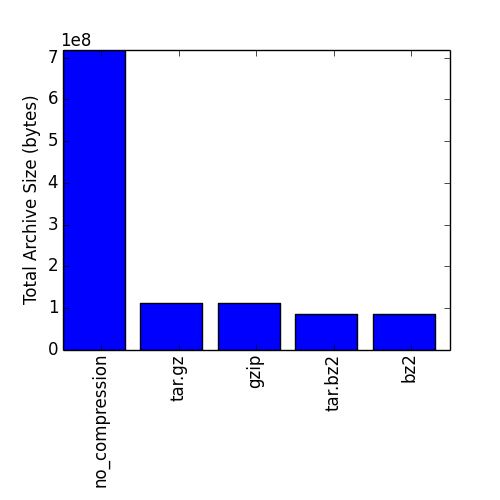
\includegraphics[width=\linewidth]{images/tas_compression.png}
      \caption{Compression comparison.}
    \end{subfigure}%
    \begin{subfigure}{.5\textwidth}
      \centering
      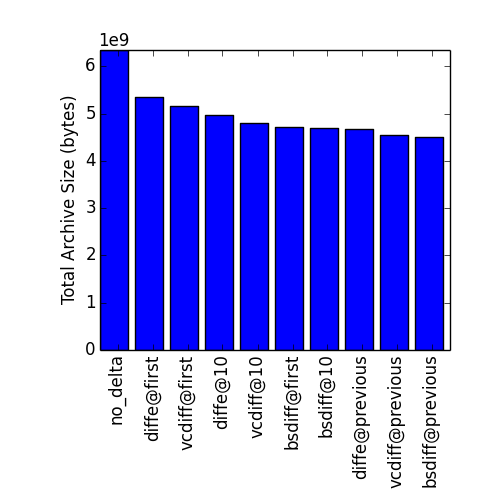
\includegraphics[width=\linewidth]{images/tas_delta.png}
      \caption{Delta comparison.}
      \label{fig:tas_delta_compression:b}
    \end{subfigure}
    \caption{Total archive size for different delta and compression strategies.}
    \label{fig:tas_delta_compression}
    \end{figure}

    \begin{figure}
    \centering
    \begin{subfigure}{.5\textwidth}
      \centering
      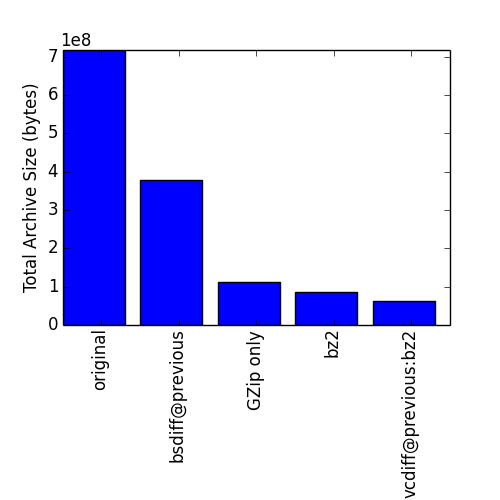
\includegraphics[width=\linewidth]{images/tas_best.png}
      \caption{Total archive size for different delta and compression strategies.}
      \label{fig:tas_best}
    \end{subfigure}%
    \begin{subfigure}{.5\textwidth}
      \centering
      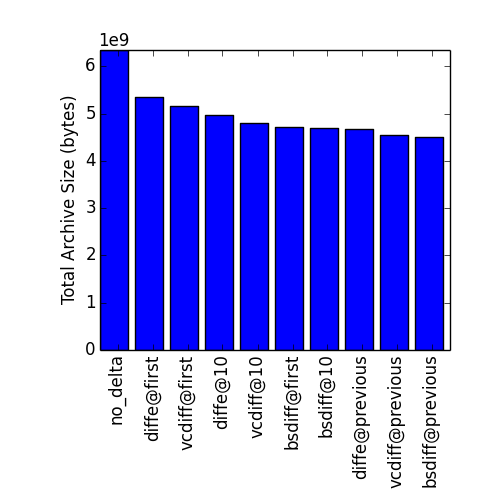
\includegraphics[width=\linewidth]{images/tas_delta.png}
      \caption{Delta comparison.}
      \label{fig:tas_delta_compression:b}
    \end{subfigure}
    \caption{Total archive size for different delta and compression strategies.}
    \label{fig:tas_delta_compression}
    \end{figure}

    We see above that the bzip2 compression algorithm produces a smaller archive than gzip, in our direct comparison bzip2 compresses our data set down to $\bzipvsgzippct\%$ of the size of gzip. In fact, bzip2 tends to more optimally compress data than gzip in many benchmarks\footnotemark. However, those benchmarks show that bzip2 achieves its compression at a slower speed than gzip. There is a trade-off to be made between storage space and time.

    \footnotetext{e.g. \url{http://compressionratings.com/sort.cgi?txt1.brief+4np2}}

    \begin{enumerate}
    \item what are the pros and cons of each strategy. e.g. speed, partitioning, do we gain little over the other strategies in terms of size but lose on speed?
    \item additionally:
    \begin{enumerate}
    \item average size of warc record types, before and after.
    \item counts of warc record types
    \item percentage space taken up by each type
    \item savings introduced by compression, why not compress the other types?
    \item compression performance by content type
    \item refer to content analysis for frequencies of content type. e.g. is it worth finding an algorithm that compresses images really well? or can we ignore them because HTML and its high change frequency trump image for storage issues.
    \end{enumerate}
    \end{enumerate}

  \subsection{Content Analysis}

    Figure~\ref{fig:file_changes_per_day} shows the number of files that changed in the archive per day. The data is split into two parts for clarity. The split is made on the day that GitHub pages launched their new naming scheme, projectname.github.io on 5 May 2013. Previously the naming scheme had been projectname.github.com. Our data crawl did not consider projects that had kept the old naming scheme. In the first $\iostarted$ days the average number of files changing per day was $\meanfilechangesfirst$, in the last $\afterio$ that increases to $\meanfilechangeslast$.

    % TODO: Insert more meaningful analysis of change frequency. Is there a strong correlation? Can we say something like 'the average domain will update at least one page every X days'? DO we see an increase in change frequency over time? Is this explained by an increase in suitable projects over time? Can we correct for this?

    \begin{figure}
    \centering
    \begin{subfigure}{.5\textwidth}
      \centering
      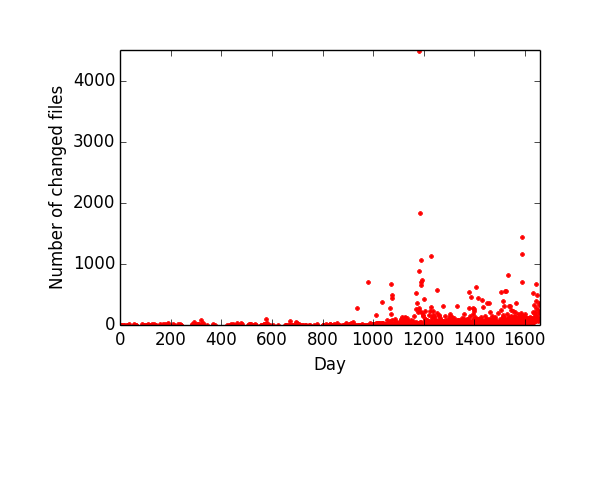
\includegraphics[width=\linewidth]{images/file_changes_per_day_first.png}
      \caption{During the first \iostarted{} days.}
    \end{subfigure}%
    \begin{subfigure}{.5\textwidth}
      \centering
      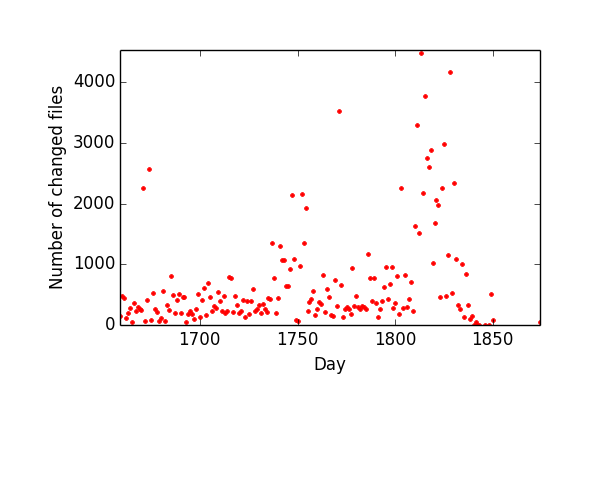
\includegraphics[width=\linewidth]{images/file_changes_per_day_last.png}
      \caption{During the last \afterio{} days.}
    \end{subfigure}
    \caption{Number of files that have changed in the archive per day.}
    \label{fig:file_changes_per_day}
    \end{figure}

    Each file change is an observation of a single file's contents differing from a previous crawl. This means that if a HTML file and a CSS file were updated simultaneously, we would record two changes. This might not align with an archivist's view of what a webpage change would be. Instead, they might expect to record a single change for updates made in a short period of time, no matter how many files were edited. In addition, we iterate through every commit made to the project but changes are only made public for every push. There may be several commits made to a project before a push. Considering this, we can instead assume that a maximum of one change is made to a domain per day. Figure~\ref{fig:domain_changes_per_day} shows the number of domains that change in the archive per day. During the first segment we see an average of $\meandomainchangesfirst$ domains changing per day, in the second segment this is $\meandomainchangeslast$.

    \begin{figure}
    \centering
    \begin{subfigure}{.5\textwidth}
      \centering
      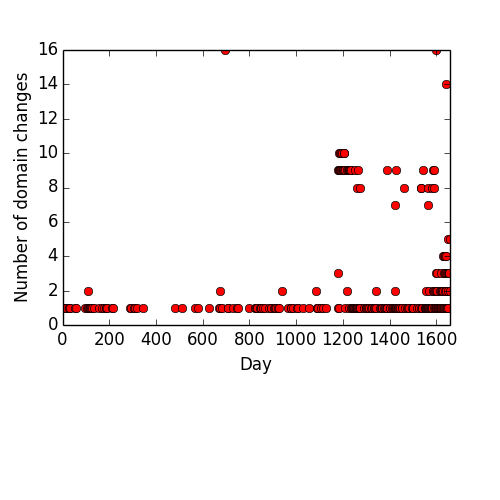
\includegraphics[width=\linewidth]{images/domain_changes_per_day_first.png}
      \caption{During the first \iostarted{} days.}
    \end{subfigure}%
    \begin{subfigure}{.5\textwidth}
      \centering
      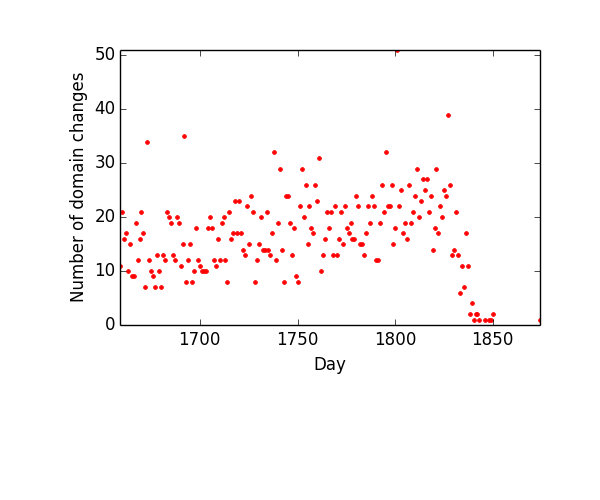
\includegraphics[width=\linewidth]{images/domain_changes_per_day_last.png}
      \caption{During the last \afterio{} days.}
    \end{subfigure}
    \caption{Number of domains that have changed in the archive per day.}
    \label{fig:domain_changes_per_day}
    \end{figure}

    Figure~\ref{fig:uris_per_domain} shows the number of URIs observed in each domain. Figure~\ref{fig:uris_per_domain:a} shows the total number of URIs ever observed at a domain. Figure~\ref{fig:uris_per_domain:b} shows the mean number of URIs observed at each domain over all crawls. The largest domain, \largestdomainname{}, has $\largestdomaintotal$ total URIs, we observed $\largestdomainmean$ of those URIs, on average, when we crawled it. The smallest domain, \smallestdomainname{}, has $\smallestdomaintotal$ URIs, $\smallestdomainmean$ on average.

    \begin{figure}
    \centering
    \begin{subfigure}{.5\textwidth}
      \centering
      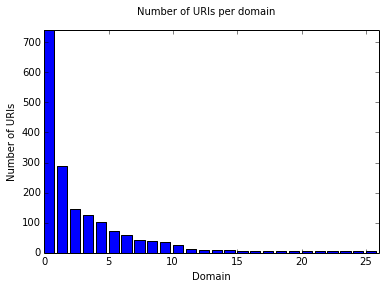
\includegraphics[width=\linewidth]{images/uris_per_domain.png}
      \caption{Total URIs.}
      \label{fig:uris_per_domain:a}
    \end{subfigure}%
    \begin{subfigure}{.5\textwidth}
      \centering
      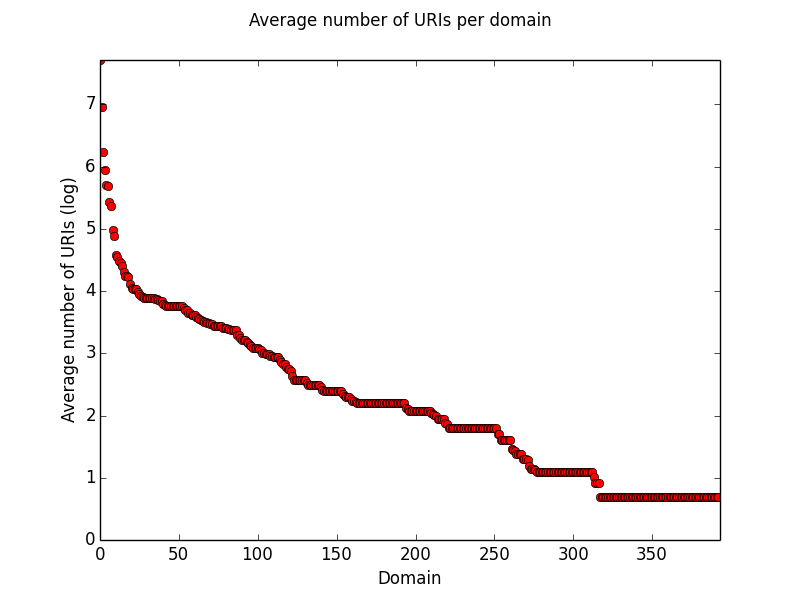
\includegraphics[width=\linewidth]{images/uris_per_domain_avg.png}
      \caption{Average URIs.}
      \label{fig:uris_per_domain:b}
    \end{subfigure}
    \caption{Number of URIs observed at each domain.}
    \label{fig:uris_per_domain}
    \end{figure}

\section{Experiment: National Archive Collection}

  \begin{enumerate}
  \item Get data from major collection
  \item BL, archive.org, etc.
  \item Apply best strategy from previous section
  \item What real-world savings can we demonstrate?
  \end{enumerate}

\section{Conclusion}

  The defaults in the WARC standard do not take advantage of the fact that many documents on the web will have many minor changes made to them over time. By using a delta algorithm as well as a compression algorithm we can reduce the total archive size by nearly half again.


\end{document}
